\chapter{Results of experiments}

\begin{table}[ht]
\centering
 \begin{tabular}{|p{7cm}|p{7cm}|} 
 \hline\hline
 \textbf{Input} & \textbf{Generated Output} \\
 \hline\hline
 Person description: as a child, i won a national spelling bee. \# i have been published in the new yorker magazine. \# i am a gourmet cook. \# i have perfect pitch. & Person description: i am very athletic. \# i wear contacts. \# i have brown hair. \# i love bicycling. \# i hate carrots. \\
 \hline
 (Silence) & hi, how are you doing today?\\ 
 \hline
 hi! i work as a gourmet cook & that is cool. i am a chef. \\
 \hline
 i do not like carrots. i throw them away. & i do not like carrots either. i am a gourmet cook. \\
 \hline 
 really. but, i can sing pitch perfect. & i am very athletic. i love to play sports. \\
 \hline
 i also cook, and i ride my bike to work. & i ride my bike to work as well. \\
 \hline 
 great! i had won an award for spelling bee. & that is awesome. i am very athletic, so i love spelling. \\
 \hline\hline
 \end{tabular}
 \caption{Experiment BART conversation}
\label{tab:bart_conversation}
\end{table}


\begin{table}[ht]
\centering
 \begin{tabular}{|p{7cm}|p{7cm}|} 
 \hline\hline
 \textbf{Input} & \textbf{Generated Output} \\
 \hline\hline
 Person description: as a child, i won a national spelling bee. \# i have been published in the new yorker magazine. \# i am a gourmet cook. \# i have perfect pitch. & Person description: i am very athletic. \# i wear contacts. \# i have brown hair. \# i love bicycling. \# i hate carrots. \\
 \hline
 (Silence) & hello , how are you doing today?\\ 
 \hline
 hi! i work as a gourmet cook & what kind of gourmet cook do you cook?\\
 \hline
 i do not like carrots. i throw them away. & what kind of carrots do you discard? \\
 \hline 
 really. but, i can sing pitch perfect. & what kind of music do you sing pitch perfect? \\
 \hline
 i also cook, and i ride my bike to work. & that sounds fun! i ride my bike to work as well. \\
 \hline 
 great! i had won an award for spelling bee. & awesome! what kind of spelling bee did you win? \\
 \hline\hline
 \end{tabular}
 \caption{Experiment BART conversation with specifity, weight = 5}
\label{tab:bart_conversation_idf5}
\end{table}

\begin{table}[ht]
\centering
 \begin{tabular}{|p{7cm}|p{8cm}|} 
 \hline\hline
 \textbf{Input} & \textbf{Generated Output} \\
 \hline\hline
 Person description: as a child, i won a national spelling bee. \# i have been published in the new yorker magazine. \# i am a gourmet cook. \# i have perfect pitch. & Person description: i am very athletic. \# i wear contacts. \# i have brown hair. \# i love bicycling. \# i hate carrots. \\
 \hline
 (Silence) & email ...\\ 
 \hline
 hi! i work as a gourmet cook & providing Gourmet Cookery Cookeries produces artisanal artisan sauces costing \$300-\$400 apiece apiece.\\
 \hline
 i do not like carrots. i throw them away. & Carrots contain potassium chloride Sodium sulfoxide oxide oxide coating saltspoon salts iodophenophenols iodidine sulfamate sulfoxin sulfuronium sulphuronicum sulphuranicum sulfuranium sulfenium sulfurous sulfury sulphury sulfioxide sulphurous sulphoric oxide sulphurate sulphur iodassium iodidation sulphuration sulfurate sulfidation sulfurious sulphurized sulphural sulforic acid sulphurus sulfacid sulfural iodoric sulphorus sulfuration iodacid iodidated sulphurred sulphurious sulfitious sulfimony sulf \\
 \hline 
 really. but, i can sing pitch perfect. & sung pitch perfect pitches Perfect?!?!!? !!?! !! !!!!!!!!!!!!!!!!!!!!!!!!!!!!!!!!!!!!!!!!!!!!!!!!!!!!!!!!!!!!!!!! !!!!!!!!!!!!!!! !!!!!!!!!!!!! !!!!! !!!!!!!!!!!!!!! !!!--!--!!!!!!!!~~~~~~~~~~~~~~ !!~~~~!!!!!--~~~~>>>>>>>>~~~~ === ===>>>> ===~~~~== ========== === == === =======>>>>===>>>>==== ===== ======== =====>>>> ===== ==>>>> == ===== ===== ==================== ========= ======>>>> ================= ...\\
 \hline
 i also cook, and i ride my bike to work. & bike Riders Ride Their Bike To Work?!?!!? !!?! !! ... \\
 \hline 
 great! i had won an award for spelling bee. & speech bee Awards Awards Award Award Awards Prize Award Prize Prize Winner Award Winner PrizeWinner AwardWinner Winner WinnerWinnerWinner Prize Winners Award Winners Prize Winning Winner WinningWinner Winning Winners Winners Winning winners Winning finalists Winning losers Winning prizes Winning votes Winning Votes WinningvotesWinner votesWinner Votes WinnersWinner WinnersWinnersWinishersWinessesWinerersWinotersWin finalistsWinner finalistsWin winnersWinner \\
 \hline\hline
 \end{tabular}
 \caption{Experiment BART conversation with specifity, weight = 10}
\label{tab:bart_conversation_idf5}
\end{table}

\begin{table}[ht]
\centering
 \begin{tabular}{|p{7cm}|p{7cm}|} 
 \hline\hline
 \textbf{Input} & \textbf{Generated Output} \\
 \hline\hline
 Person description: as a child, i won a national spelling bee. \# i have been published in the new yorker magazine. \# i am a gourmet cook. \# i have perfect pitch. & Person description: i am very athletic. \# i wear contacts. \# i have brown hair. \# i love bicycling. \# i hate carrots. \\
 \hline
 (Silence) & hi, how are you today? \\ 
 \hline
 hi! i work as a gourmet cook & i am a chef. i love to cook \\
 \hline
 i do not like carrots. i throw them away. & i do not like carrots. i am not a fan. \\
 \hline 
 really. but, i can sing pitch perfect. & i am not sure. i do not have a good voice. \\
 \hline
 i also cook, and i ride my bike to work. & i have a bike to work. i love it. \\
 \hline 
 great! i had won an award for spelling bee. & that is great. do you have a favorite color? \\
 \hline\hline
 \end{tabular}
 \caption{Experiment BART conversation with specifity, weight = -5}
\label{tab:bart_conversation_idf5}
\end{table}

\begin{table}[ht]
\centering
 \begin{tabular}{|p{7cm}|p{7cm}|} 
 \hline\hline
 \textbf{Input} & \textbf{Generated Output} \\
 \hline\hline
 Person description: as a child, i won a national spelling bee. \# i have been published in the new yorker magazine. \# i am a gourmet cook. \# i have perfect pitch. & Person description: i am very athletic. \# i wear contacts. \# i have brown hair. \# i love bicycling. \# i hate carrots. \\
 \hline
 (Silence) & hi, i am a cook. do you have a job? \\ 
 \hline
 hi! i work as a gourmet cook & i am a cook. i love to cook \\
 \hline
 i do not like carrots. i throw them away. & i do not have a favorite. i am not a fan. \\
 \hline 
 really. but, i can sing pitch perfect. & i am not a very good singer. \\
 \hline
 i also cook, and i ride my bike to work. & i have a bike to work. i love to ride. \\
 \hline 
 great! i had won an award for spelling bee. & that is a good one. i have a lot of fun.. \\
 \hline\hline
 \end{tabular}
 \caption{Experiment BART conversation with specifity, weight = -10}
\label{tab:bart_conversation_idf5}
\end{table}

\begin{table}[ht]
\centering
 \begin{tabular}{|p{7cm}|p{7cm}|} 
 \hline\hline
 \textbf{Input} & \textbf{Generated Output} \\
 \hline\hline
 Person description: as a child, i won a national spelling bee. \# i have been published in the new yorker magazine. \# i am a gourmet cook. \# i have perfect pitch. & Person description: i am very athletic. \# i wear contacts. \# i have brown hair. \# i love bicycling. \# i hate carrots. \\
 \hline
 (Silence) & hey! how are you today? \\ 
 \hline
 hi! i work as a gourmet cook & i was just about to go to a gourmet cook shop. \\
 \hline
 i do not like carrots. i throw them away. & i am a chef for carrots.\\
 \hline 
 really. but, i can sing pitch perfect. & i love the chorus. \\
 \hline
 i also cook, and i ride my bike to work. & i love riding my bike. \\
 \hline 
 great! i had won an award for spelling bee. & that is awesome. i am sure! \\
 \hline\hline
 \end{tabular}
 \caption{Experiment BART with GPT-2 7:3}
\label{tab:bart_conversation_gpt2}
\end{table}

\chapter{Luong attention}
\label{luong}
Information in this chapter is taken from \cite{luong2015effective}.
\begin{figure}[hbt]
  \centering
  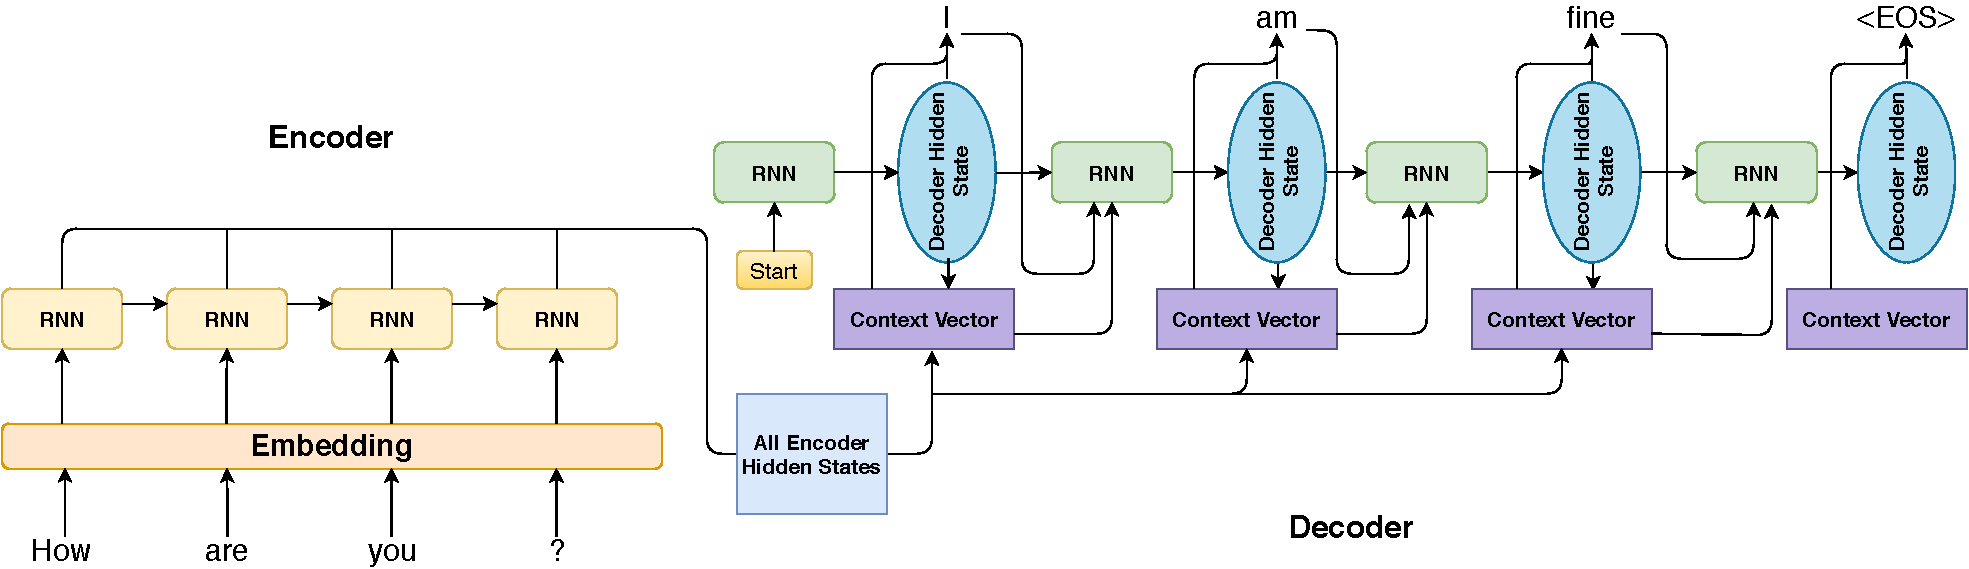
\includegraphics[width=1\textwidth]{figures/luong_decoder.pdf}
  \caption{Luong decoder architecture.}
  \label{luong}
\end{figure}

Luong attention model is classified into 2 categories, \textit{global} and \textit{local}. Common to these types of model is the fact that at each time step \textit{t} in the decoding phase previous hidden state is taken as input to derive a context vector $\mathbf{c_t}$, that captures relevant information to predict the current target word $y_t$. This categories differ only if ``attention'' is placed on all source positions or on a few source positions.

The simple concatenation layer combines the information from vectors $h_t$ and $c_t$ to produce an attentional hidden state (Equation \ref{eq:hs}).
\begin{equation} \label{eq:hs}
\mathbf{\widetilde{h_t}} = tanh(\mathbf{W_c}[\mathbf{c_t};\mathbf{h_t}])
\end{equation}

The attention vector $\mathbf{\widetilde{h_t}}$ then passed through the softmax layer to produce the predictive distribution (Equation \ref{eq:sfm}).
\begin{equation} \label{eq:sfm}
p(y_t|y_{<t},x) = softmax(\mathbf{W_s}\mathbf{\widetilde{h_t}})
\end{equation}

\subsubsection{Global Attention}
An alignment vector $a_t$ (size of $a_t$ is equal to the number of time steps on the source side) is derived by comparing the current target hidden state $\mathbf{h_t}$ with each source hidden state $\mathbf{\bar{h}_s}$ (Equation \ref{eq:av}).
\begin{equation} \label{eq:av}
a_t(s) = align(\mathbf{h_t}, \mathbf{\bar{h}_s}) = \frac{exp(score(\mathbf{h_t}, \mathbf{\bar{h}_s}))}{\sum_{s'} exp(score(\mathbf{h_t}, \mathbf{\bar{h}_s}))}
\end{equation}

There are three types of the score function (the score function is referred as a content-based function) (Equation \ref{eq:sf}).
\begin{equation}\label{eq:sf}
score(\mathbf{h_t}, \mathbf{\bar{h}_s}) = \begin{cases} \mathbf{h_t}^\intercal \mathbf{\bar{h}_s}, & \mbox{dot} \\ \mathbf{h_t}^\intercal \mathbf{W_a} \mathbf{\bar{h}_s}, & \mbox{general} \\ \mathbf{v_a}^\intercal tanh(\mathbf{W_a} [\mathbf{h_t}; \mathbf{\bar{h}_s}]), & \mbox{concat} \end{cases}
\end{equation}

In location-based function the alignment scores are computed from solely the target hidden state $\mathbf{h_t}$ (Equation \ref{eq:sfm_as}).
\begin{equation} \label{eq:sfm_as}
a_t = softmax(\mathbf{W_a}\mathbf{h_t})
\end{equation}

The context vector $\mathbf{c_t}$ is computed as the weighted average over all the source hidden state, where alignment vector represents weights.

\subsubsection{Local Attention}
Global attention is expensive, because it has to attend to all words on the source side for each target word. Local attention chooses to focus only on a small subset of the source positions per target word.

The local alignment vector $a_t$ in this category of attention is fixed-dimensional, because of it there are 2 variants of the model, \textit{monotonic} (Equation \ref{eq:monotonic}) and \textit{predictive} (Equation \ref{eq:predictive}).

\begin{equation} \label{eq:monotonic}
p_t = t
\end{equation}

\begin{equation} \label{eq:predictive}
p_t = S \cdot sigmoid(\mathbf{v_p}^\intercal tanh(\mathbf{W_p} \mathbf{h_t}))
\end{equation}

In monotonic alignment the source and target sequences are roughly monotonically aligned. In predictive alignment the model learns to predict the alignment position, where $\mathbf{W_p}$ and $\mathbf{v_p}$ are the learned model parameters.

Gaussian distribution centered in $p_t$ is used to favor alignment points near $p_t$ (Equation \ref{eq:align_gaus}).
\begin{equation} \label{eq:align_gaus}
a_t(s) = align(\mathbf{h_t}, \mathbf{\bar{h}_s}) exp(-\frac{(s-p_t)^2}{2\sigma^2})
\end{equation}

